\section{C’est dans la boite}


\subsection{Au rapport !}
Nos héros quittant Jebble son contacté par leur faction.

\subsubsection{Empire}
\begin{quotebox}
    \nameref{sec:garan-keggle}: Au rapport ! Comment avance vos recherches sur l’artefact ?
\end{quotebox}
Les joueurs racontent\ldots
\begin{quotebox}
    \nameref{sec:garan-keggle}: La "Boite de Jebble"\ldots Ca ne me dit rien ! Mais allez voir \nameref{sec:fane-peturri} sur \textbf{Muunilinst}, c’est un historien de l’Empire, ami de notre Empereur, il pourra certainement vous aider. Je vais le prévenir de votre visite et je vous transfère ses coordonnées.
\end{quotebox}

Les héros se rendent donc sur \textbf{Muunilinst} (normalement) et rencontrent \nameref{sec:fane-peturri}. Ce dernier les invite chez lui, leur offre le thé et les reçoient bien.
\begin{quotebox}
    \nameref{sec:fane-peturri}: Garan m’a prévenu de votre arrivée mais il ne m’a pas dit quel était le but de votre visite ? En quoi puis-je aider l’empire ?
\end{quotebox}
Les héros devraient donc lui parler de la fameuse boite de Jebble qui est en réalité \nameref{sec:oubliette-de-dreypa}.

\begin{quotebox}
    \nameref{sec:fane-peturri}: Il me semblait bien qu’il y avait un rapport entre l’oubliette et cette Boite ! Il y a quelques temps, suite à une réquisition d’oeuvres d’art pour le compte de l’empire, je suis tombé sur un enregistrement holo qui parlait de cette boite. D’après ce que disant l’enregistrement, mais il date maintenant de plusieurs mois, la \textbf{Boite de Jebble} se trouve sur le \nameref{sec:uhumele} un cargo qui verse dans le commerce et la contrebande de babioles diverses. Son capitaine, \nameref{sec:schurk-heren} est un Yarkora qui se méfie de tout le monde en général et en particulier de l’Empire.

    Le dernier port d’attache que je lui connais est \textbf{Pizkoss}, il est certainement en train d’essayé de refourguer sa marchandise !
\end{quotebox}

\subsubsection{Rebelion}
\begin{quotebox}
    \nameref{sec:lindi-dangon}: Bonjour, je viens aux nouvelles, comment se passe la recherche de l’artéfact ? Vous avez besoin de quelque chose ?
\end{quotebox}

Les joueurs racontent\ldots

\begin{quotebox}
    \nameref{sec:lindi-dangon}: La \textbf{Boite de Jebble}, ça me dit quelque chose, attendez une seconde\ldots 

    \textit{Lindi disparait de l’écran un instant puis revient}

    \nameref{sec:lindi-dangon}: Effectivement, un Jedi en parle dans un de ses rapports. \nameref{sec:dass-jennir}, il n’est pas très précis dans son rapport, mais vous devriez aller le voir. Il est en retraite sur \textbf{Muunilinst}. Je vous fais suivre les coordonnées où vous le trouverez, soyez respectueux et diplomates ! Rappelez vous que c’est un Jedi !
\end{quotebox}

Les héros se rendent donc sur \textbf{Muunilinst} (normalement) pour rencontrer \nameref{sec:dass-jennir}. Dass Jennir se montre tout d’abord froid et distant
\begin{quotebox}
    \nameref{sec:dass-jennir}: C’est pour quoi ? Si c’est encore pour réparer votre moissonneuse, revenez plus tard, je suis occupé là.
\end{quotebox}

Aux héros de se montrer diplomate pour l’amadouer ! Quand c’est fait. Ils lui parlent de la Boite de Jebble. En entendant ce nom, le visage de Dass Jennir marque un sentiment de souffrance et de regret. C’est manifestement un souvenir douloureux pour lui.
\begin{quotebox}
    \nameref{sec:dass-jennir}: Oui, je me souviens de ça ! Je ne l’ai pas vu personnellement mais elle faisait partie de l’inventaire de l’\nameref{sec:uhumele} quand je suis passé à son bord pour une mission. L’équipage du vaisseau avait à son bord cette chose, au dernière nouvelles ils partaient sur \textbf{Pizkoss} pour tenter de trouver un acheteur pour cette cargaison.

    Vous devez savoir que déjà à l’époque, l’Empire recherchait hardement cette cargaison, c’est d’ailleurs ce qui explique qu’il ne l’ai toujours pas revendue. 

    Le capitaine du cargo s’appelle \nameref{sec:schurk-heren} je vais vous dire où le trouver sur \textbf{Pizkoss} mais je ne viendrais pas avec vous, j’en ai fini avec tout ça.
\end{quotebox}

Quand \nameref{sec:schurk-heren} fait escale sur \textbf{Pizkoss}, il a l’habitude de dépenser ses crédit chez \nameref{sec:queen-jool}.

\newpage
\subsection{Pizkoss’ Paradise}
Pizkoss était un Monde du Noyau. En tant que tel, le commerce y est très prospère et on y retrouve à peu près toutes les races possible. Toutes sortes de transaction et on lieu des plus légale au plus douteuses. En tant que planète du noyau elle est surveillé par l’Empire.

\nameref{sec:queen-jool} est la propriétaire d’une cantina libertine sur \textbf{Pizkoss}, le \textbf{Paradise}. C’est un club "select" où l’on ne rentre que sur invitation. Il ne faut pas chercher à rentrer de force sous prétexte de se faire explicer violament et d’attirer par la même l’attention de l’Empire. Diplomatie et astuce (déguisement, soudoiement, propositions indessante \ldots) sont de rigueur. Une fois à l’interieur, attention de ne pas faire de vagues ! Au moindre problèmes, vigiles et \nameref{sec:storm-trooper}s débarquent et enferment tout le monde.\\

\noindent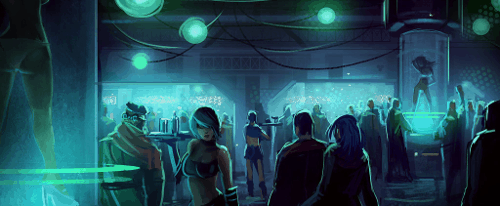
\includegraphics[width=\linewidth]{_img/dos-au-muur/places/paradise-club.png}\\

\'A l’intérieur la salle se présente comme un stripbar classique. Un bar sur la droite, une estrade au fond avec un podium qui avance sur la moitié de la pièce. Des îlos plus privés tout au tour et des salons privatif sur la gauche. 

Les héros ne savent pas à quoi ressemble \nameref{sec:schurk-heren} ils n’ont que son nom, à eux de le retrouver. En vrai il se trouve dans l’un des salons privés où il profite d’une dance avec \textbf{Na’tuna}, une charmante Twi’lek en tenue légère.

Quand les héros rentrent dans le salon, Schurk est un peu surpris, Na’Tuna reste imperturbable, professionalisme avant tout.

\begin{quotebox}
    \nameref{sec:schurk-heren}: Ben faut pas vous géner ! Décidément tout se perd, les bonnes manières y compris ! Je ne sais pas ce que vous me voulez mais vous ne pensez pas que ça peut attendre que la dame est terminée ?
\end{quotebox}

Gérez Schurk en fonction du comportement de vos héros, quand ils se mettent à discuter :

\begin{quotebox}
    \nameref{sec:schurk-heren}: Bon, maintenant que l’on est entre nous, en quoi puis-je vous aider ?
    \ldot
    \nameref{sec:schurk-heren}: Humm, alors comme ça cet innestimable et antique coffre vous intéresse ?
\end{quotebox}

\clearpage
\subsection{l’Uhumele}\label{sec:uhumele}
\noindent
\includegraphics[width=\textwidth]{_img/songes-de-l-uhumele/uhumele-pano.png}

L'Uhumele est un vaisseau cargo de classe inconnue, actif notamment pendant et après la Guerre des Clones. Son capitaine est le Yarkora Schurk-Heren. On ignore quand et dans quelles conditions Schurk-Heren devint capitaine de l’Uhumele et comment son équipage le rejoignit. Ce qui est sûr, c'est qu’il a de bonnes raisons de détester la République et de craindre l’Empire qui lui succède.

L’Uhumele est avant tout un vaisseau de contrebande, comme un bon nombre de cargos en apparence en règle. De ce fait, il est doté d’un armement susceptible de pouvoir le sortir des situations délicates dans lesquelles il se fourre. L’une de ces armes est un bras rétractable situé sous le ventre de l’appareil, au bout duquel se trouve une petite tourelle blaster, ressemblant à celle des Canonnières clones. Bien que cette tourelle permette d’avoir un très vaste angle de tir, elle rend la situation du tireur précaire car très exposé. 

\hspace{12em}
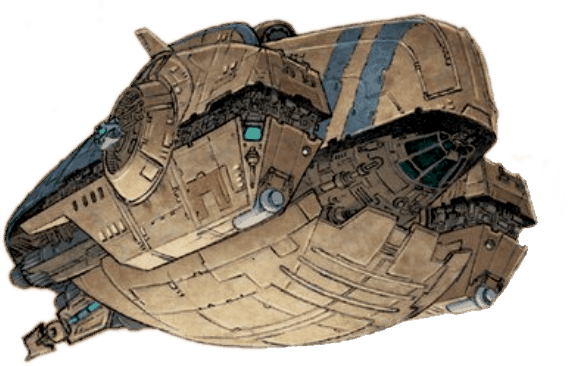
\includegraphics[width=0.8\textwidth]{_img/songes-de-l-uhumele/uhumele.png}
%   Ici une idée est qu'au moment de quitté la planète pour l'étape suivante, les héros se retrouvent pris au piège par des troupes de l'empire qui on pris leur vaisseau en otage. Histoire de varier l'aventure. On peut même se mettre une petite baston spaciale.

% La suite c’est qu'il faut retrouver la boite avant que quelqu'un d'autre ne mette la main dessus (l'Empire ou un rival de Palpatine). Mais c'est raté, c'est les méchant d'en face qui récupèrent en premier et qui l'ouvre.

% scénario suivant et final, les méchant tendent un piège aux héros grace à Céleste mais les gentils parviennent à libérer Celeste et à remettre l'amulette dans l'oubliette. Cette dernière est récupérer par la faction des héros et conservée à l'abris.